% !TEX root = main.tex
\documentclass[11pt]{article}

\usepackage[a4paper,margin=1in]{geometry}
\usepackage[T1]{fontenc}
\usepackage{lmodern}
\usepackage{microtype}
\usepackage{amsmath,amssymb,mathtools}
\usepackage{booktabs}
\usepackage{array}
\usepackage{multirow}
\usepackage{tabularx}
\usepackage{float}
\usepackage{enumitem}
\usepackage{xcolor}
\usepackage{tikz}
\usetikzlibrary{arrows.meta,positioning,fit,calc}
\usepackage{graphicx}
\usepackage{natbib}
\usepackage[hidelinks]{hyperref}

\newcolumntype{L}[1]{>{\raggedright\arraybackslash}p{#1}}

\newcommand{\pp}{\,\mathrm{pp}}
\newcommand{\ro}{\textsc{Relational-Orbit}}
\newcommand{\rootonly}{\textsc{Root}}
\newcommand{\mapped}{\textsc{Mapped}}
\newcommand{\qwen}{Qwen2.5}

\title{Canonicalizing Option-Permuted Views Improves Matched-Compute Multiple-Choice Inference}
\author{Author names and affiliations to be added}
\date{}

\begin{document}
\maketitle

\begin{abstract}
 Large language models are sensitive to the coordinate system used to express a multiple-choice problem: reordering answer options can change the emitted label even when the underlying question is unchanged. Standard self-consistency treats such outputs as samples in one label space and therefore cannot distinguish semantic agreement from coordinate agreement. We study a controlled alternative, \ro{} inference, which applies the exact inverse of a known option permutation to every transformed-view answer before aggregating a smoothed categorical distribution. On the first Qwen2.5-3B public-benchmark block, mapped inference improved matched-compute accuracy by 17.71 percentage points. Two independent Qwen2.5-3B follow-up blocks retained a 7.29-point gain across 384 new questions. A shared-question panel spanning Qwen, Llama, Phi, Mistral and Gemma checkpoints showed positive fixed-model average effects, and a further shared block gave a 9.38-point gain for Mistral-7B. Correct maps consistently outperformed randomized maps, while Qwen2.5-7B ceiling effects, a negative Gemma-MMLU result, harder synthetic tasks and affine transformations exposed clear boundaries. The evidence supports positive average transfer across the tested fixed panel, not universal benefit for every model, benchmark or transformation; mapped test-time reinforcement-learning (TTRL) remained exploratory on real benchmarks.
\end{abstract}

\section{Introduction}

Multiple-choice evaluation is attractive for language-model research because it provides a discrete decision target, reproducible scoring and broad coverage of reasoning and knowledge tasks. Yet the target is not only a semantic choice. A model must also emit a coordinate label such as ``A'' or ``D'', and the relationship between the semantic option and that label changes when the options are permuted. Empirical studies have documented substantial sensitivity to option order and position, even when the question content is held fixed \citep{zheng2023selectors,pezeshkpour2024order}. This creates a failure mode for test-time aggregation: two answers can be semantically identical while carrying different surface labels, or can agree in label while referring to different options.

For example, suppose the canonical answer is option 2, and a cyclic rotation moves that option to position 0. A model that emits ``0'' for the rotated prompt has selected the same semantic answer as a model that emits ``2'' for the canonical prompt. Pooling the two raw labels treats them as disagreement; applying the known inverse rotation converts both observations to canonical option 2 before aggregation. This distinction between semantic identity and label identity is the object tested here.

Self-consistency addresses a related problem by sampling multiple reasoning paths and marginalizing their answers \citep{wang2023selfconsistency}. Its usual aggregation, however, assumes that all samples already inhabit a common answer coordinate system. A prompt ensemble that changes option order violates that assumption. Permutation self-consistency has also been studied for listwise ranking, where reordered candidate lists are aggregated to reduce order effects \citep{tang2024middle}; listwise marginalization does not, by itself, provide the exact inverse map needed for a multiple-choice answer label.

Here we test whether known relational structure can be used as an inference-time alignment operation. We generate matched samples from an identity prompt and three cyclic option rotations. Each transformed answer is mapped back to the canonical option index before a full-support log-opinion pool is formed. The method is deliberately narrow: it assumes a known, finite option permutation and does not claim to solve arbitrary prompt inconsistency. The central question is whether exact alignment improves accuracy beyond root-only self-consistency when the number of generated completions is held fixed.

We evaluate this question in an evidence ladder. A CPU simulator tests the intended recovery mechanism and coherently wrong controls. A Qwen2.5-3B model is evaluated on synthetic arithmetic and three public benchmarks, followed by a disjoint Qwen2.5-7B confirmation. We then run a shared-question block across Qwen2.5-3B, Qwen2.5-7B and Llama-3.2-3B, and a further fixed panel of Phi-3.5-mini, Mistral-7B-Instruct-v0.3 and Gemma-2-2B. The latter panel was frozen before candidate generations and tests transfer across five model families. We also report compute scaling, hard-vote and randomized-map controls, label-free selective risk, and matched-compute TTRL adaptation diagnostics.

The contribution has two parts: an auditable inference-time estimator that canonicalizes transformed answers before pooling, and an empirical characterization of when that estimator helps or fails. The resulting claim is bounded: the method shows positive average transfer across the tested fixed model panel, while medium-difficulty arithmetic, affine transformations, some high-ceiling benchmark blocks and real-benchmark policy adaptation define important limits.

\section{Related work}

\paragraph{Self-consistency and test-time sampling.}
Self-consistency samples multiple reasoning paths and aggregates their final answers, improving chain-of-thought reasoning without changing model parameters \citep{wang2023selfconsistency}. Our method retains the matched-compute sampling principle but changes the order of operations: a known transformation is inverted before the samples are pooled. This makes the transformation part of the estimator rather than an unmodelled source of output variation.

\paragraph{Multiple-choice order sensitivity.}
Large language models are not robust multiple-choice selectors, and their answer distributions can depend on option position \citep{zheng2023selectors}. Controlled studies of option-order sensitivity provide a direct motivation for treating answer labels as coordinates rather than semantic objects \citep{pezeshkpour2024order}. We use the same kind of option reorderings as a controlled intervention, but retain the exact correspondence between transformed and canonical options for aggregation.

\paragraph{Permutation-aware aggregation.}
Permutation self-consistency improves listwise ranking by marginalizing over candidate-list orderings \citep{tang2024middle}. The present setting differs in both object and operation: the output is a four-way answer label, the transformations form a known cyclic action, and the inverse action is applied to each sampled label before probability pooling. Randomized inverse maps and unmapped-view baselines separate this relational signal from diversity generated by merely changing the prompt.

\section{Method}

\subsection{Task formulation and relational views}

For a question with four canonical options, let the answer space be
\[
    \mathcal{A}=\{\varnothing,0,1,2,3\},
\]
where $\varnothing$ denotes a parser failure and the integer indices denote the four canonical options. Let $G=C_4$ be the cyclic group of option rotations. For each $g\in G$, the question is rendered with options transformed by $g$, and the model emits $R$ sampled labels $y_{g,1},\ldots,y_{g,R}$. The known inverse map $g^{-1}$ sends a valid transformed label back to its canonical index and leaves $\varnothing$ unchanged.

The experimental pipeline is shown in Fig.~\ref{fig:pipeline}. The identity view is retained as the root coordinate system. The three non-identity views are generated with the same question stem and answer content, but with cyclically shifted option positions. The transformations disperse every fixed-position shortcut over all four canonical candidates.

\begin{figure}[t]
\centering
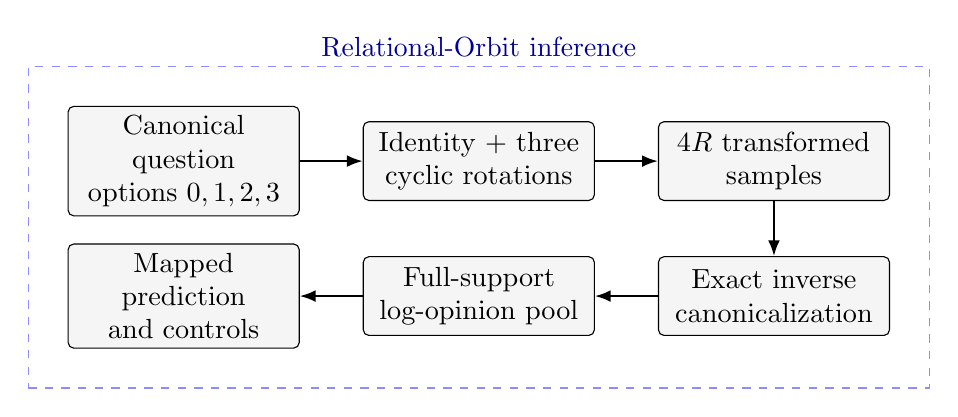
\begin{tikzpicture}[
  node distance=7mm and 8mm,
  box/.style={draw, rounded corners=2pt, align=center, minimum height=10mm, text width=27mm, fill=gray!8},
  arrow/.style={-{Latex[length=2mm]}, thick}
]
\node[box] (q) {Canonical question\\options $0,1,2,3$};
\node[box, right=of q] (views) {Identity + three\\cyclic rotations};
\node[box, right=of views] (gen) {$4R$ transformed\\samples};
\node[box, below=of gen] (map) {Exact inverse\\canonicalization};
\node[box, left=of map] (pool) {Full-support\\log-opinion pool};
\node[box, left=of pool] (pred) {Mapped prediction\\and controls};
\draw[arrow] (q) -- (views);
\draw[arrow] (views) -- (gen);
\draw[arrow] (gen) -- (map);
\draw[arrow] (map) -- (pool);
\draw[arrow] (pool) -- (pred);
\node[fit=(q)(views)(gen)(map)(pool)(pred), draw=blue!45, dashed, inner sep=5mm, label={[blue!60!black]above:Relational-Orbit inference}] {};
\end{tikzpicture}
\caption{Inference-time exact option-space alignment. Transformed-view samples are mapped to a shared canonical coordinate system before aggregation. The root-only baseline spends the same total generation budget on the identity prompt.}
\label{fig:pipeline}
\end{figure}

\subsection{Canonical log-opinion pooling}

For each view, mapped sample counts are smoothed over the complete support. With $n_g(a)$ occurrences of answer $a$ among $R$ samples and smoothing constant $\alpha=1$,
\[
 p_g(a)=\frac{n_g(a)+\alpha}{R+\alpha|\mathcal{A}|}.
\]
The canonical log-opinion pool is
\[
 q(a)=\frac{\exp\left(\frac{1}{|G|}\sum_{g\in G}\log p_g(a)\right)}
 {\sum_{b\in\mathcal{A}}\exp\left(\frac{1}{|G|}\sum_{g\in G}\log p_g(b)\right)}.
\]
The prediction is $\arg\max_{a\in\{0,1,2,3\}}q(a)$; the parse-failure symbol remains in the normalization and is never silently discarded. Ties use the lowest answer index.

The matched-compute root baseline uses $|G|R=16$ samples from the identity prompt and majority vote. The unmapped baseline pools transformed labels without applying inverse maps. For the randomized-map control, the identity inverse is retained and each non-identity inverse is composed with an independently sampled random permutation of the four labels. Thus the control preserves the generated text and the generation budget while destroying the known relational correspondence.

\subsection{Test-time reinforcement-learning adaptation diagnostic}

The parameter-updating experiments use the same views but replace the final pooled prediction with leave-one-out soft rewards. For a rollout $r$ in view $g$, its reward is the pooled probability assigned to its mapped answer after that rollout is removed from its own view. Rewards are centered within each prompt. The policy update maximizes the full completion sequence log-probability weighted by the centered reward and adds a KL penalty to the frozen reference model:
\[
 \mathcal{L}= -\frac{1}{B}\sum_i A_i\log\pi_\theta(y_i\mid x_i)
 +\beta\,\mathrm{KL}(\pi_\theta\,\|\,\pi_{\mathrm{ref}}),
\]
with low-rank adaptation (LoRA) rank 8 \citep{hu2022lora}, learning rate $10^{-5}$, $\beta=0.02$, one on-policy pass and target modules $q_{\mathrm{proj}}$ and $v_{\mathrm{proj}}$. Root test-time reinforcement learning (TTRL) receives the same sequence budget on the identity prompt. These experiments are reported as exploratory because the real-benchmark diagnostic was not decisive.

\subsection{Label-free reliability}

For each mapped prediction, we recompute the prediction after omitting each transformed view in turn. The primary stability score is the fraction of leave-one-view-out predictions equal to the full prediction. A secondary margin is the difference between the two largest pooled answer probabilities. Examples are ranked by decreasing stability, then margin, then content hash, without using labels. Accuracy and risk are reported at 25\%, 50\%, 75\% and 100\% coverage.

\section{Experimental design and statistical analysis}

\subsection{Models, benchmarks and compute}

All language-model experiments used FP16 inference on one NVIDIA RTX 3090 with 24 GB memory. Unless otherwise stated, prompts used temperature 0.8, top-$p$ 0.95, maximum 192 new tokens, four cyclic views and four samples per view. The primary benchmarks were ARC-Challenge validation \citep{clark2018arc}, OpenBookQA validation \citep{mihaylov2018openbookqa} and MMLU test \citep{hendrycks2021mmlu}, restricted to eligible four-option questions. Dataset snapshots were mirrored locally, fingerprinted and recorded in every manifest.

The initial public-benchmark transfer used Qwen2.5-3B-Instruct; a disjoint content-hash block was used for Qwen2.5-7B-Instruct \citep{qwen2025technical}. The first shared block evaluated Qwen2.5-3B-Instruct, Qwen2.5-7B-Instruct and Llama-3.2-3B-Instruct \citep{dubey2024llama} on the same 192 questions. A frozen extension evaluated Phi-3.5-mini-Instruct \citep{abdin2024phi}, Mistral-7B-Instruct-v0.3 \citep{jiang2023mistral} and Gemma-2-2B-it \citep{team2024gemma2} on those identical question hashes. Later independent-sample experiments evaluated two new Qwen2.5-3B blocks, one new Qwen2.5-7B block and a second 192-question block shared exactly across Gemma, Phi and Mistral. All model checkpoints were fixed before their corresponding generations.

\subsection{Question blocks and preregistration}

Question selection was deterministic using content hashes. The initial 3B and 7B transfer blocks, the adaptation training and evaluation blocks, and the original Llama block were disjoint. The first shared block removed all prior hashes before selecting 64 questions per benchmark with seed 20260817. The two Qwen2.5-3B follow-up blocks used new sample offsets and were combined only after all three benchmarks in both blocks finished. The Qwen2.5-7B precision block explicitly excluded every prior 7B manifest. The 20260828 Gemma/Phi/Mistral block likewise excluded the first shared panel; manifest audits confirmed that all three models received the same 64 questions per benchmark. Thus cross-model averages use paired shared questions, whereas within-model replication pools disjoint questions.

\subsection{Primary estimands and reporting}

For every question, the primary paired contrast was mapped correctness minus matched-compute root correctness. The map-control contrast was mapped correctness minus the mean correctness of 20 randomized inverse-map controls generated from the same transformed samples. The main text reports sample size, Root and Mapped accuracy, percentage-point differences, map controls and frozen gate decisions. To keep the enlarged result tables readable, numerical uncertainty intervals are archived in the machine-readable supplementary analyses rather than repeated in the main text. All gate decisions still use the prespecified paired bootstrap calculations. For shared blocks, questions are resampled within benchmark strata and the same indices are applied to every fixed model. Model checkpoints are fixed estimands, not random draws from all language models.

The shared-block paper gate required a positive fixed-model-average uncertainty result, at least two of three nonnegative model effects, no model wholly negative under the paired analysis, a map-control effect of at least 5 points with positive uncertainty bounds, truth support at least 0.80 and parse failure at most 0.10 for every model, plus successful audits. The cross-family panel added a stricter requirement that at least one new model independently exceed 3 points and pass its paired uncertainty criterion. Failed gates were retained and did not trigger tuning on their evaluation questions. Per-model and per-benchmark comparisons outside a frozen gate are descriptive and are not multiplicity-adjusted.

\section{Results}

We organize the experiments as an evidence ladder: controlled recovery, public-benchmark transfer, matched cross-model comparisons, independent new-sample replication, and finally compute, reliability and failure-boundary analyses. Accuracy and effect values below are percentages or percentage-point differences.

\subsection{Mechanism and synthetic recovery}

The CPU testbed first isolated the statistical mechanism from language-model behavior. With 10,000 simulated orbits, dispersed shortcut errors produced a mapped accuracy of 1.000 versus 0.125 for root-only inference (a +87.5-point contrast). A stable shortcut produced 0.020 mapped accuracy versus 0.125 root accuracy, and a coherently wrong regime produced zero accuracy for both methods. Thus mapping can repair errors when view-specific shortcuts disperse, but cannot repair a coherent wrong mode.

The easy synthetic Qwen2.5-3B pilot reproduced the predicted recovery effect. In the confirmatory 64-orbit block, mapped pooling improved accuracy from 54.69\% to 81.25\% (+26.56 points); an independent 64-orbit replication improved accuracy from 57.81\% to 82.81\% (+25.00 points). Correct maps exceeded randomized gauges by 43.44 and 44.30 points, respectively. Truth-support coverage was at least 96.9\% and parse failure was approximately 2\% in both runs.

The preregistered medium-difficulty gate was intentionally harder: each arithmetic problem used two or three operations and moduli 11, 13, 17 or 19. One seed gave +12.50 points and the other -1.56 points; their pooled +5.47-point effect did not meet the frozen effect and map-control criteria. A post-gate easy reference reproduced a +31.25-point gain, ruling out environment drift. The medium result therefore marks a model-capability boundary rather than an implementation failure.

\begin{table}[H]
\centering\small
\caption{Synthetic recovery and transformation-family boundaries. Each model-backed row reports matched-compute accuracy and the correct-map advantage over randomized maps.}
\label{tab:synthetic}
\begin{tabular}{lrrrrr}
\toprule
Condition & $n$ & Root & Mapped & Difference & Map control \\
\midrule
Easy, seed 808 & 64 & 54.69 & 81.25 & +26.56 & +43.44 \\
Easy, seed 909 & 64 & 57.81 & 82.81 & +25.00 & +44.30 \\
Medium, seed 6808 & 64 & 31.25 & 43.75 & +12.50 & +12.27 \\
Medium, seed 6909 & 64 & 32.81 & 31.25 & -1.56 & +7.19 \\
Boolean negation & 32 & 31.25 & 37.50 & +6.25 & -0.94 \\
Affine scale + shift & 32 & 59.38 & 53.13 & -6.25 & +23.59 \\
Affine shift-only & 32 & 87.50 & 68.75 & -18.75 & +29.53 \\
\bottomrule
\end{tabular}
\end{table}

The transformation-family characterization further bounded the claim. Boolean negation was retained as a negative control because the correct-map advantage over randomized maps was -0.94 points. Affine transformations beat randomized gauges but harmed root-only accuracy, with mapped-minus-root effects of -6.25 and -18.75 points for the two affine families. Exact semantic validity of a map therefore does not guarantee a positive net accuracy effect.

\subsection{Primary public-benchmark transfer}

The first public-benchmark transfer used 64 questions per benchmark and 16 total generations per question. On Qwen2.5-3B, mapped pooling improved ARC-Challenge by 28.13 points, OpenBookQA by 10.94 points and MMLU by 14.06 points. Pooled accuracy rose from 53.65\% to 71.35\%, a +17.71-point gain, and the frozen transfer gate passed. Correct maps exceeded randomized maps by 35.63 points, showing that option diversity without the known inverse correspondence was insufficient.

The disjoint Qwen2.5-7B confirmation also passed its original gate. Root accuracy was already 79.69\%, while mapped accuracy reached 84.90\%, giving a smaller +5.21-point gain. Its +40.39-point map control remained large, consistent with a ceiling-limited accuracy effect rather than failure of the relational signal.

\begin{table}[H]
\centering\small
\caption{Initial public-benchmark transfer at two Qwen2.5 scales. Each benchmark row contains 64 questions; pooled rows contain 192 independent questions.}
\label{tab:public}
\begin{tabular}{llrrrr}
\toprule
Model & Benchmark & Root & Mapped & Difference & Map control \\
\midrule
3B & ARC-Challenge & 46.9 & 75.0 & +28.1 & +43.2 \\
3B & OpenBookQA & 75.0 & 85.9 & +10.9 & +44.8 \\
3B & MMLU & 39.1 & 53.1 & +14.1 & +18.9 \\
3B & Pooled & 53.6 & 71.4 & \textbf{+17.7} & +35.6 \\
\midrule
7B & ARC-Challenge & 90.6 & 93.8 & +3.1 & +48.8 \\
7B & OpenBookQA & 81.3 & 87.5 & +6.3 & +42.3 \\
7B & MMLU & 67.2 & 73.4 & +6.3 & +30.2 \\
7B & Pooled & 79.7 & 84.9 & \textbf{+5.2} & +40.4 \\
\bottomrule
\end{tabular}
\end{table}

\subsection{Matched cross-model transfer on a shared question block}

The first cross-model analysis evaluated Qwen2.5-3B, Qwen2.5-7B and Llama-3.2-3B on exactly the same 192 questions. Their fixed-model average gain was +3.13 points, and correct maps exceeded randomized maps by +34.67 points. The frozen shared-block gate passed. The model-level effects were heterogeneous: Qwen2.5-3B improved by +7.29 points, Qwen2.5-7B by +2.60 points, and Llama-3.2-3B by -0.52 points. The Llama result therefore remains a null boundary rather than evidence for universal transfer.

We next ran Phi-3.5-mini, Mistral-7B and Gemma-2-2B on the identical question hashes. All three point estimates were positive, yielding a +3.65-point fixed-model average and a +34.23-point map control. Truth support ranged from 94.3\% to 97.9\%, parse failure ranged from 0.5\% to 1.0\%, and the structural, overlap, symmetry and token-budget audits passed. The stricter extension gate nevertheless failed because no new model independently passed its paired criterion on this first block. This panel supports positive average transfer across the fixed checkpoints, not confirmed benefit for every checkpoint.

\begin{table}[H]
\centering\small
\caption{Matched cross-model results on one shared block of 192 independent questions. Each panel average contains 576 model--question observations, but inference preserves the 192-question pairing and treats the listed checkpoints as fixed.}
\label{tab:families}
\begin{tabular}{lrrrrl}
\toprule
Model or fixed panel & Root & Mapped & Difference & Map control & Decision \\
\midrule
Qwen2.5-3B & 62.0 & 69.3 & +7.3 & +31.6 & Descriptive \\
Qwen2.5-7B & 82.3 & 84.9 & +2.6 & +40.2 & Descriptive \\
Llama-3.2-3B & 75.0 & 74.5 & -0.5 & +32.2 & Descriptive \\
Qwen/Llama average & 73.1 & 76.2 & \textbf{+3.1} & +34.7 & Passed \\
\midrule
Phi-3.5-mini & 80.2 & 82.3 & +2.1 & +36.8 & Descriptive \\
Mistral-7B & 66.7 & 71.9 & +5.2 & +30.9 & Descriptive \\
Gemma-2-2B & 72.4 & 76.0 & +3.6 & +34.9 & Descriptive \\
Phi/Mistral/Gemma average & 73.1 & 76.7 & \textbf{+3.6} & +34.2 & Strict gate failed \\
\bottomrule
\end{tabular}
\end{table}

\subsection{Independent new-sample replication}

Independent question blocks sharpened the generalization claim (Table~\ref{tab:replication}). Two disjoint Qwen2.5-3B follow-up blocks produced gains of +6.77 and +7.81 points. Combined across 384 independent questions, Root accuracy was 59.38\% and Mapped accuracy was 66.67\%, a +7.29-point gain that passed the frozen paired criterion. By contrast, the expanded Qwen2.5-7B evidence remained ceiling limited: across its original and new blocks, Root was 84.38\%, Mapped was 84.90\%, and the +0.52-point effect did not pass.

The second block shared by Gemma, Phi and Mistral produced the clearest cross-family replication. Mistral-7B improved from 69.27\% to 78.65\% (+9.38 points) and passed its individual gate; OpenBookQA contributed the largest benchmark-level gain at +14.06 points. Phi improved by +2.60 points but did not pass individually. Gemma changed by -0.52 points overall and fell by 10.94 points on MMLU, an explicit negative model--benchmark result. Averaging the three fixed models on the 192 shared questions gave +3.82 points and a +35.37-point map control. This three-model aggregate was computed after the shared hashes were verified and is reported descriptively rather than as a preregistered gate.

\begin{table}[H]
\centering\small
\caption{Independent new-sample replication at the primary $N=16$ generation budget. The final row averages three fixed models over 192 shared questions (576 model--question observations) and is post-hoc descriptive.}
\label{tab:replication}
\begin{tabular}{lrrrrrl}
\toprule
Model or fixed panel & $n$ & Root & Mapped & Difference & Map control & Decision \\
\midrule
Qwen2.5-3B, two new blocks & 384 & 59.4 & 66.7 & \textbf{+7.3} & +30.3 & Passed \\
Qwen2.5-7B, original + new & 384 & 84.4 & 84.9 & +0.5 & +39.6 & Failed \\
Gemma-2-2B, new block & 192 & 75.5 & 75.0 & -0.5 & +32.6 & Failed \\
Phi-3.5-mini, new block & 192 & 79.2 & 81.8 & +2.6 & +37.7 & Failed \\
Mistral-7B, new block & 192 & 69.3 & 78.6 & \textbf{+9.4} & +35.8 & Passed \\
Three-model fixed average & 192 & 74.7 & 78.5 & \textbf{+3.8} & +35.4 & Descriptive \\
\bottomrule
\end{tabular}
\end{table}

\subsection{Compute scaling, pooling and label-free reliability}

The stored generations permitted $N=4/8/16$ matched-compute analyses without additional model calls. No universal monotonic budget pattern emerged (Table~\ref{tab:scaling}). Qwen2.5-3B and Mistral improved as the budget increased, Phi and Gemma had larger gains at lower budgets, and Qwen2.5-7B stayed near its high Root ceiling. The prespecified $N=16$ result remains primary; selecting each model's best budget after observing outcomes would overstate performance.

Hard vote and full-support log-opinion pooling were close across blocks, and neither uniformly dominated. We therefore retained log pooling as the primary estimator and report hard vote only as an ablation. The leave-one-view-out stability score also provided a useful label-free ranking signal. At 50\% coverage, Mapped accuracy ranged from 91.67\% to 96.88\% across the five independent analysis sets. These selective results are descriptive: labels were not used to rank examples, but performance has not been calibrated for an unseen deployment distribution.

\begin{table}[H]
\centering\small
\caption{Compute scaling and selective accuracy on the independent follow-up sets. The first three columns report Mapped minus matched-compute Root in percentage points; the last reports Mapped accuracy after retaining the 50\% most stable questions.}
\label{tab:scaling}
\begin{tabular}{lrrrr}
\toprule
Model & $N=4$ & $N=8$ & $N=16$ & Accuracy at 50\% coverage \\
\midrule
Qwen2.5-3B & +2.9 & +6.3 & +7.3 & 91.7 \\
Qwen2.5-7B & -1.0 & +0.8 & +0.5 & 96.9 \\
Gemma-2-2B & +2.6 & +4.2 & -0.5 & 92.7 \\
Phi-3.5-mini & +5.2 & +3.6 & +2.6 & 94.8 \\
Mistral-7B & +0.5 & +5.2 & +9.4 & 92.7 \\
\bottomrule
\end{tabular}
\end{table}

\subsection{Failure boundaries and exploratory adaptation}

The easy synthetic TTRL study used five independent seeds, 16 unlabeled training orbits and 512 sequences per method per seed. Across 304 fresh evaluation orbits, mapped TTRL exceeded matched-compute root TTRL by +5.65 points under an equal-seed estimate, and all five seed-level effects were positive. The mapped method also exceeded the unadapted base by +7.03 points, with finite and small training KL.

The real-benchmark adaptation diagnostic used 18 unlabeled training questions and 96 untouched evaluation questions. Mapped TTRL exceeded root TTRL by +2.08 points, with benchmark-level effects of -0.78 on ARC-Challenge, +3.91 on OpenBookQA and +3.13 on MMLU. It did not pass the frozen paired uncertainty criterion, so no multi-seed real-benchmark adaptation expansion was run. TTRL is therefore exploratory rather than a primary empirical claim.

Difficulty and transformation controls define a separate boundary. The medium synthetic gate failed despite one positive seed, Boolean negation did not beat the randomized-map control, and affine transformations reduced accuracy relative to Root by 6.25 and 18.75 points. These negative results rule out the stronger claim that any semantically valid transformation, model or reasoning distribution benefits from relational pooling.

\section{Discussion}

The experiments support a simple interpretation: when model errors contain a coordinate-dependent component, exact inverse alignment converts several transformed views into evidence about one semantic answer. The randomized-map controls are important here. Transformed prompts alone were not sufficient; the known map produced a large and consistent advantage over random inverse gauges across Qwen, Llama, Phi, Mistral and Gemma panels.

The effect was heterogeneous rather than model universal. Qwen2.5-3B retained a +7.29-point gain over two independent blocks, and Mistral-7B provided a separate +9.38-point cross-family replication. Qwen2.5-7B, however, changed by only +0.52 points after its evidence was expanded to 384 questions, consistent with limited headroom at 84.38\% Root accuracy. Gemma was neutral overall on its new block and negative on MMLU. The scaling analysis adds an important qualification: more samples strengthened Qwen2.5-3B and Mistral but not Phi, Gemma or Qwen2.5-7B. Budget and baseline accuracy influence the opportunity for alignment, but they do not fully explain the observed model--task interactions.

The experiments also distinguish inference-time alignment from policy adaptation. Mapped rewards improved easy synthetic adaptation across all five seeds, but the real-benchmark diagnostic failed its frozen paired criterion. The policy update introduces additional sources of variance, including sparse training questions, model-specific optimization behavior and a mismatch between the training reward and final benchmark accuracy. We therefore treat TTRL as a secondary direction rather than the central contribution.

Several limitations are intrinsic to the study. All public tasks use four-option multiple choice, and the maps are cyclic option permutations. The candidate checkpoints are fixed rather than sampled from a population of language models, so fixed-model averages apply only to the tested panel. Shared blocks permit high-sensitivity matched comparisons, whereas only the later blocks test transfer to new task content. Some model--benchmark pairs were negative, including Llama on the first shared block and Gemma on the new MMLU block. The current study also lacks a unified head-to-head evaluation against every permutation-aware aggregation method. Finally, the affine controls show directly that exact knowledge of a transformation does not guarantee improved task accuracy.

The practical implication is narrower and more useful than a universal claim. Exact relational alignment is a parameter-free inference wrapper that can improve average matched-compute multiple-choice accuracy and can provide a label-free confidence signal for selective prediction, although it increases generation cost by evaluating multiple prompt views. Its use should therefore be accompanied by task-specific validation, a randomized-map control, an explicit compute budget and comparison with the strongest available permutation-aware baseline. The current evidence motivates such validation rather than replacing it.

\section{Conclusion}

We introduced an auditable inference-time procedure that maps option-permuted model outputs into a shared canonical space before pooling. Exact alignment improved matched-compute accuracy by 7.29 points across 384 independent Qwen2.5-3B follow-up questions and by 9.38 points on an independent Mistral-7B block; both passed their frozen paired criteria. Fixed-model panels showed smaller positive average effects and large advantages over randomized maps, while Qwen2.5-7B, Gemma-MMLU, harder synthetic tasks and affine transformations established clear boundaries. The evidence supports a useful inference-time wrapper for validated four-option settings, not a universal improvement claim. TTRL adaptation on real benchmarks remains exploratory.

\section*{Methods availability and reproducibility}

The repository contains frozen protocols, source code, test suites, raw parsed records, manifests, environment descriptions and model-output audit reports. The primary inference implementation uses Python, NumPy, PyTorch and Transformers; parameter updates use PEFT LoRA. All final records include question content hashes, exact permutations, parsed samples, root samples, parse-failure rates, truth-support status and completion-token totals. The originating remote run reported 25 passing tests for the cross-family panel and the local project suite reported 30 passing tests. The current draft still requires author-supplied author names, affiliations, funding, ethics/declaration text and final verification of publisher metadata for references before submission.

\bibliographystyle{plainnat}
\bibliography{references}

\clearpage
\appendix
\section{Complete experimental inventory}

\begin{table}[ht]
\centering\small
\caption{Inventory of the frozen experiments reported in this manuscript.}
\label{tab:inventory}
\begin{tabularx}{\textwidth}{@{}L{0.27\textwidth}L{0.20\textwidth}>{\raggedright\arraybackslash}X@{}}
\toprule
Block & Independent units & Purpose and decision \\
\midrule
CPU simulator & 10,000 orbits & Mechanism, dispersed shortcut and coherent-wrong controls \\
Easy synthetic inference & 64 + 64 orbits & Confirmatory and replication recovery tests \\
Medium synthetic inference & 64 + 64 orbits & Preregistered capability-boundary gate; failed \\
Transformation families & 32 per family & Boolean negative control and affine boundary characterization \\
Qwen2.5-3B transfer & 64 per benchmark & Public-benchmark transfer gate; passed \\
Qwen2.5-7B confirmation & 64 per benchmark & Disjoint model-scale confirmation; passed \\
Synthetic adaptation & 5 seeds & Matched-compute mapped versus root TTRL; positive exploratory result \\
Real adaptation & 18 train, 96 eval & Frozen policy-update diagnostic; paired criterion not passed \\
Original Llama gate & 64 per benchmark & First cross-family diagnostic; paired criterion not passed \\
Shared three-model block & 192 shared questions & Qwen/Llama fixed-model paper gate; passed \\
New family panel & 192 shared questions per model & Phi/Mistral/Gemma average transfer; strict individual gate not passed \\
Qwen2.5-3B follow-up 1 & 192 questions & Independent replication block; individual gate not passed \\
Qwen2.5-3B follow-up 2 & 192 questions & Independent replication block; passed \\
Qwen2.5-7B precision block & 192 questions & New disjoint block; combined 384-question gate not passed \\
Gemma-2-2B new block & 192 questions & Smaller-model replication; overall gate not passed \\
Phi/Mistral new shared block & 192 shared questions per model & Mistral passed; Phi did not pass \\
Three-model new-block average & 192 shared questions & 576 model--question observations; descriptive post-hoc summary \\
\bottomrule
\end{tabularx}
\end{table}

\section{Machine-readable result inventory}

The complete old-and-new result index is provided in the supplementary
experiment CSV, with a readable Markdown companion at the repository root.
Shared-block analyses are stored under \texttt{outputs/paper\_scale\_shared/}
and \texttt{outputs/cross\_family\_panel\_20260817/}; the corrected new-block
fixed-model analysis is stored in the dated follow-up reanalysis JSON. Exact
filenames and source paths are indexed in the supplementary CSV. The main
tables round accuracy and effects to one decimal percentage point. Full-precision
estimates, paired uncertainty analyses, benchmark-level rows, parse diagnostics
and manifest hashes remain in the archived outputs.

\end{document}
